\documentclass[12pt,titlepage,a4paper]{report}
% Texte
\usepackage[utf8]{inputenc}
\usepackage[T1]{fontenc}
\usepackage[french]{babel}
\usepackage{lmodern}
\usepackage{float}
\usepackage{enumitem}
\usepackage{minted}
% Pour les checkmarks
\usepackage{pifont}
\usepackage{amssymb}
% Pour des \hline en gras
\usepackage{makecell}
% Numéroter les chapitres à partir de chaque début de partie
\makeatletter\@addtoreset{chapter}{part}\makeatother

% Mise en page
\usepackage{url}
\usepackage[top=2.1cm,bottom=2cm,left=1cm,right=1cm]{geometry}
\usepackage{hyperref}
\hypersetup{
    colorlinks=false,
    pdfborder={0 0 0},
}
\usepackage{multirow}

% TOC
\usepackage[french]{minitoc}
\setcounter{tocdepth}{2}
\setcounter{minitocdepth}{2}
\setlength{\mtcindent}{0pt}

% Images
\usepackage{float}
\usepackage{wrapfig}
\usepackage{graphicx}
% Pour inclure des pages PDF
\usepackage[final]{pdfpages}

% Couverture
\usepackage{templateINSA}
\initINSA

\title{Reconnaissance de caractères et detection de langue}
\author{Manon \bsc{Ansart}\\ Anthony \bsc{Courtin}}

\renewcommand\soustitre{Rapport de projet}
\renewcommand\infoBig{Projet d'Approfondissement et d'Ouverture}
\renewcommand\infoSmall{ASI4 2014-2015}
\newcommand{\code}[1]{\texttt{#1}}
\newcommand{\hlineGras}{\Xhline{2\arrayrulewidth}}

\def\changemargin#1#2{\list{}{\rightmargin#2\leftmargin#1}\item[]}
\let\endchangemargin=\endlist 

\begin{document}
	\titleINSA{15}{images/fond.jpeg}{0}{0}{300}{\href{http://img0.gtsstatic.com/wallpapers/92e875b279aa0e52dc1b5cc12443416a_large.jpeg}{\textcolor{white}{CC - Istockphotos}}}

	\dominitoc
	\tableofcontents

	\chapter{Introduction}
		Le but initial de ce projet était de travailler avec la librairie Olena d'Epita afin de détecter des photos dans des images de documents. Après le téléchargement et la compilation de la librairie, nous avons tenté de la tester et de rechercher les fonctions utiles pour l'application que nous voulions en faire. Nous avons découvert que la librairie était bien plus complexe que ce que nous pensions, et qu'elle ne fournissait pas de fonction permettant de trouver directement une photo dans une image. Nous avons donc décidé de choisir un autre sujet, toujours dans le cadre de la reconnaissance d'image de document. Pendant ce Projet d'Approfondissement et d'Ouverture, nous allons utiliser la bibliothèque ocropus pour reconnaître les caractères à partir d'une image de documents puis en détecter la langue grâce au module de détection de langue cld2 développé par google.

	\chapter{Compréhension des outils}
		\section{Ocropus}
		\subsection{Généralités}
	OCRopus est un logiciel libre de reconnaissance optique de caractères (ROC) ou optical character recognition (OCR) en anglais. Il a pour but de pouvoir être utilisé à la fois par des chercheurs et des entreprises\cite{articleOCRopus}, c'est pourquoi il a été développé sous licence Apache 2, qui permet une utilisation commerciale facile. 

	OCRopus permet d'utiliser plusieurs modules de reconnaissance de texte. En particulier, il implémente Tesseract, qui est considéré comme un des modules les plus exactes dans le domaine des logiciels libres. Ces performances se rapprochent de celles des modules commerciaux peu connus.

\subsection{Fonctionnement}
	OCRopus, comme n'importe quel logiciel d'OCR, fonctionne selon 5 étapes principales \cite{articleOCRopus} : Le pré-traitement, l'analyse de page, la reconnaissance des caractères, le post-traitement puis la mise en forme du résultat

	\subsubsection{Pré-traitement}
		Cette étape a pour but de traiter l'image d'entrée afin de faciliter les étapes suivantes. Cela implique par exemple de redresser une image inclinée, de travailler sur le contraste... OCRopus fourni une toolbox pour les images en noir et blanc ou niveau de gris.

	\subsubsection{Analyse de page}
		Une fois l'image optimisée pour le traitement, elle est découpée en lignes de texte. Pour cela, OCRopus recherche d'abord la présence de colonnes, puis découpe chacune de ces colonnes en lignes. Ces lignes pourront ensuite être traitées séparément

	\subsubsection{Reconnaissance de caractère}
		Les lignes en sortie de l'étape précédente sont analysées afin d'en reconnaître les différents caractères. Pour se faire, les images de caractères sont analysées une à une et comparées par différentes méthodes a des images de caractères connus dans une base de donné. Le ou les caractères les plus proches sont choisis. C'est dans cette partie que Tesseract est utilisé.

	\subsubsection{Post-traitement}
		Une analyse statistique est ensuite utilisée pour améliorer le résultat et lever les éventuelles ambiguïtés. Des dictionnaires sont utilisés pour calculer la probabilité de séquences de lettres, ce qui permet de poser un modèle linguistique utilisé dans cette étape.

	\subsubsection{Mise en forme}
		Les lignes ayant été analysées une par une, une dernière étape est nécessaire afin de mettre en forme les différents résultats obtenus afin d'obtenir une résultat final unique : une page html contenant le texte de sortie. Un script bash nous permet de convertir cet page html en un fichier txt. 


\subsection{Résultats}
	
	Nous avons tenté d'utiliser OCRopus pour obtenir le texte présent dans différentes images. 

	\begin{figure}[H]
		\centering
		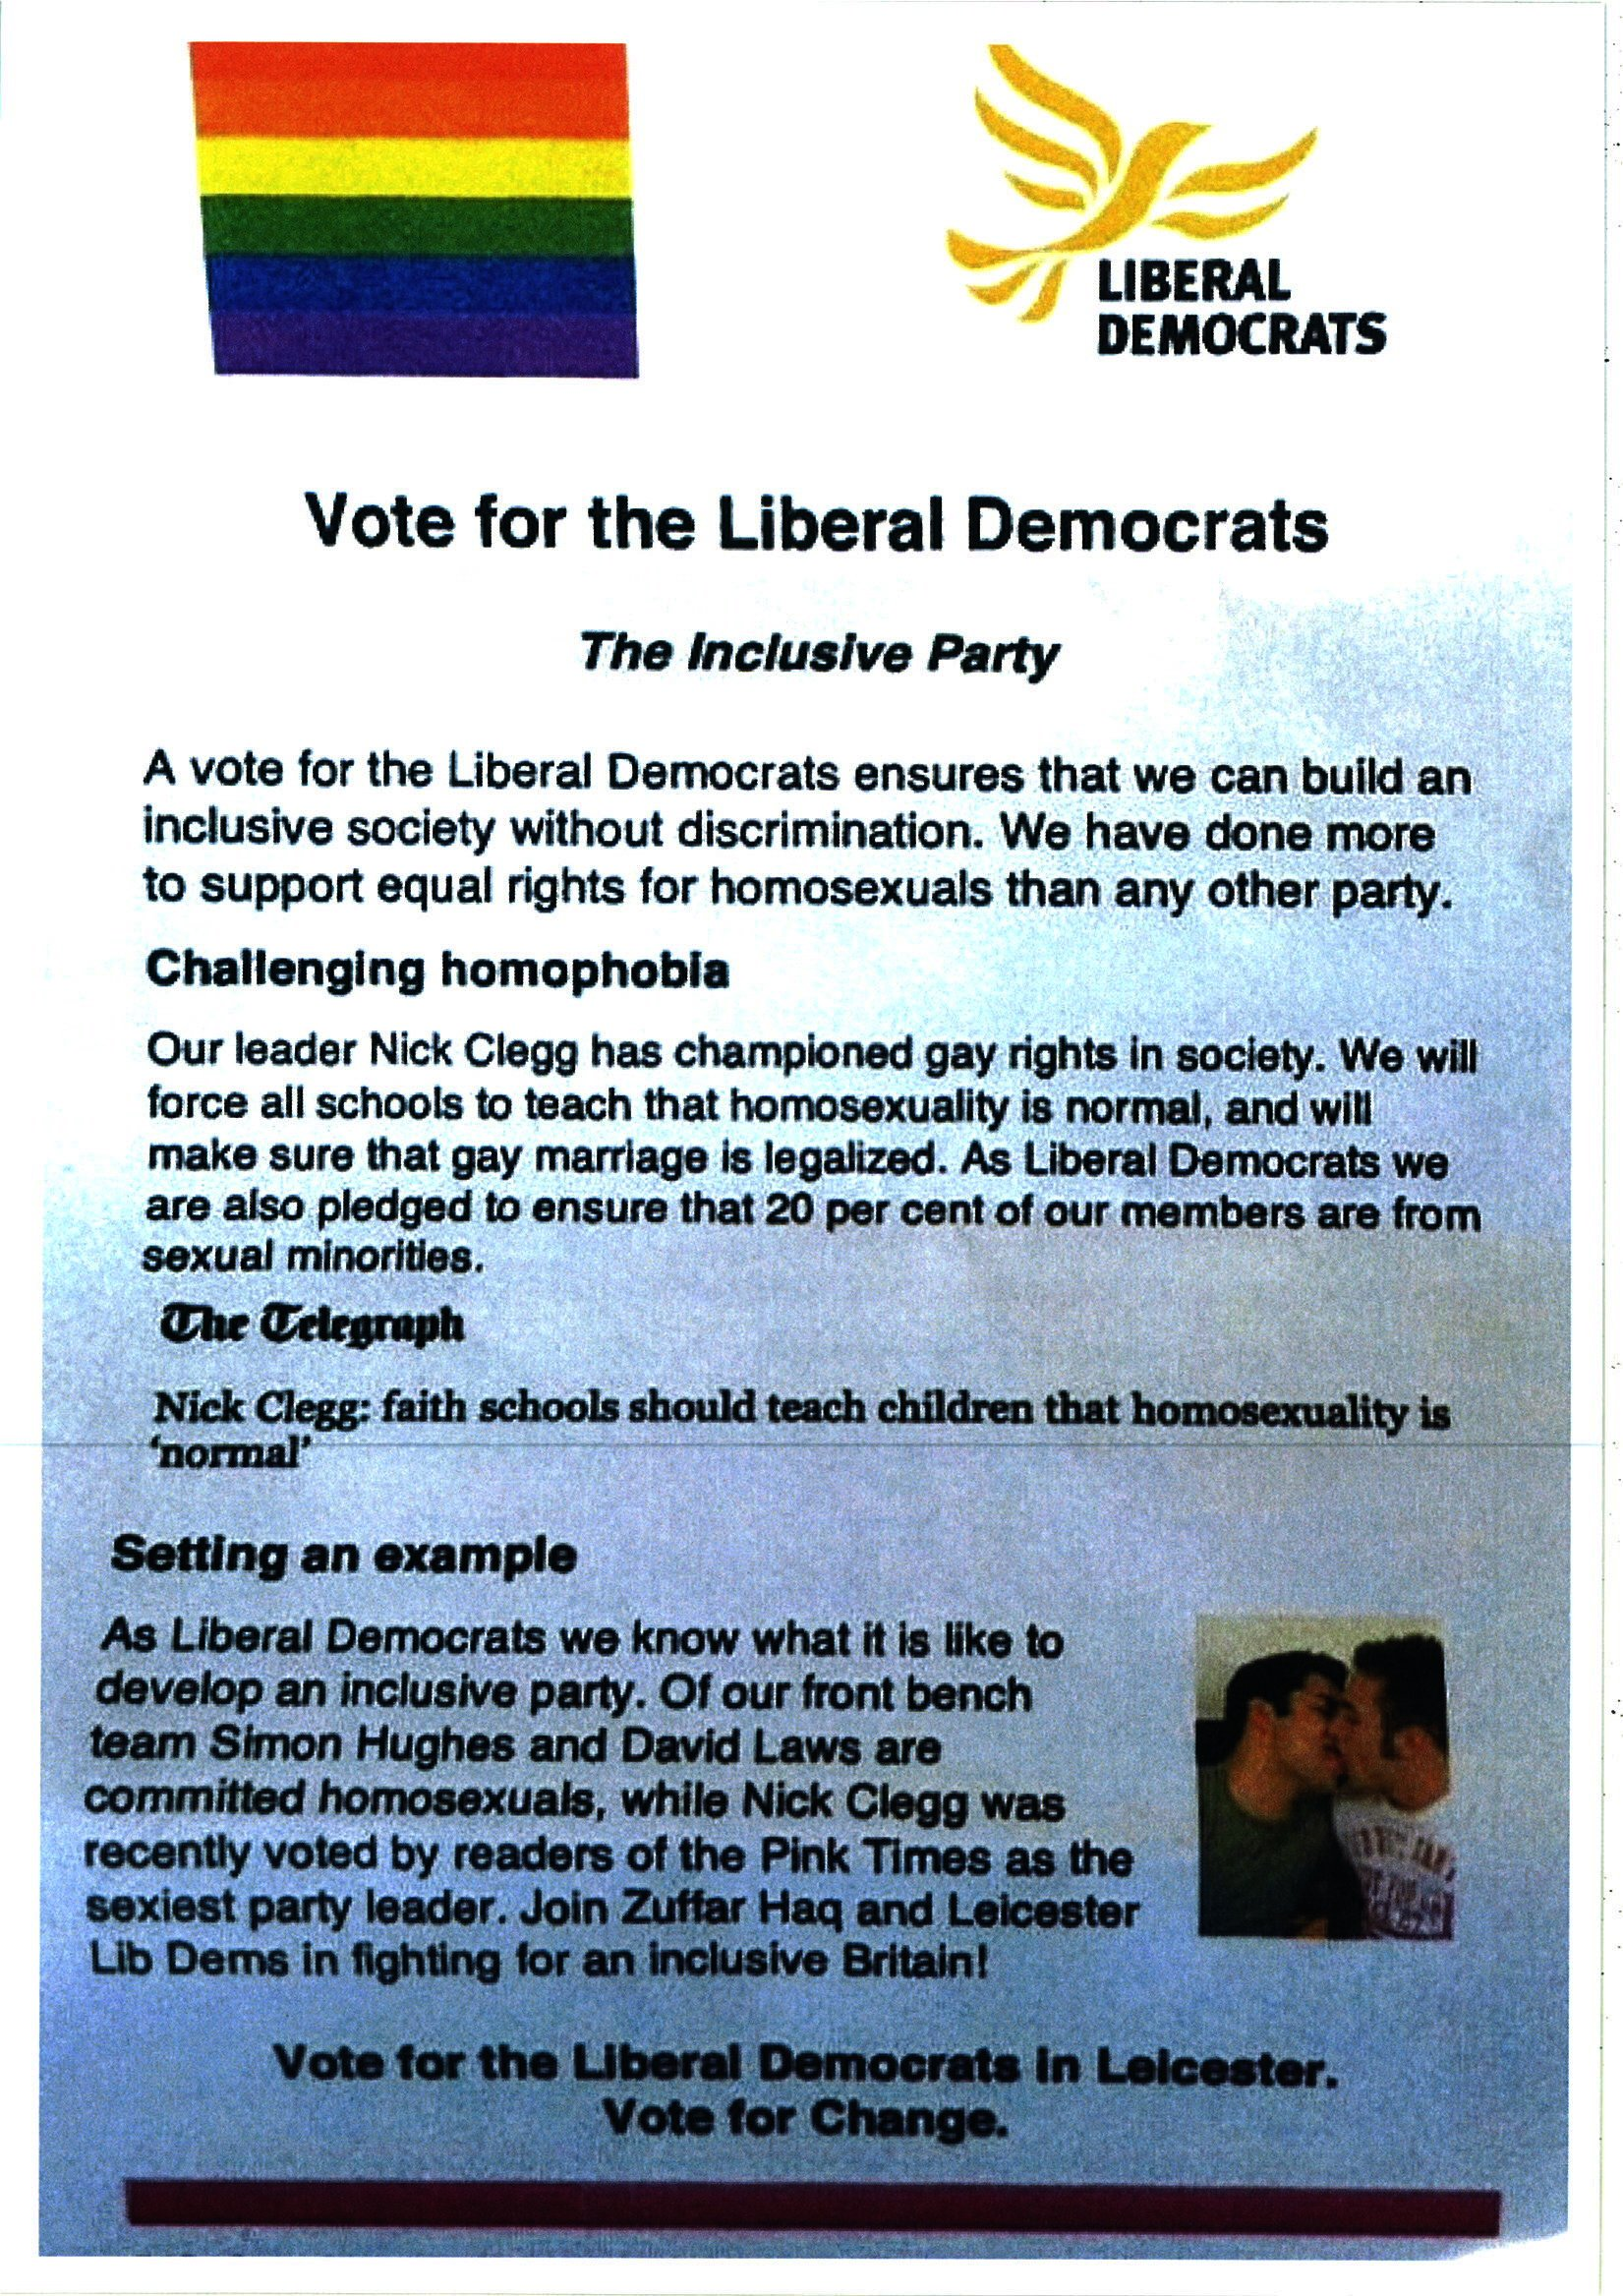
\includegraphics[scale=0.4]{images/FJEZNU.jpg}
		\caption{Image à traiter par OCRopus}
		\label{fig:image}
	\end{figure}

	\begin{figure}[H]
		\centering
		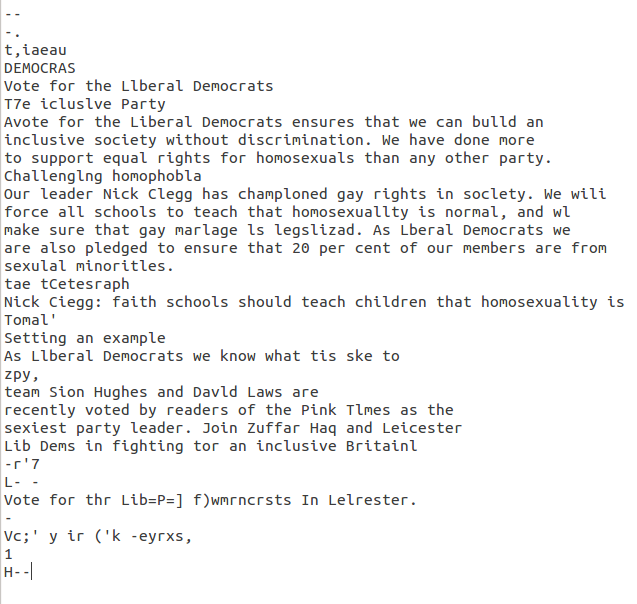
\includegraphics[scale=0.6]{images/FJEZNU_result.png}
		\caption{Texte trouvé par OCRopus}
		\label{fig:resultat}
	\end{figure}

	Avec cette image, on remarque que les lettre se ressemblant (i et l) sont souvent confondues, et que la qualité de l'image est importante : le bas de la page, moins bien éclairé, est mal reconnu et le mot "normal", situé sur la pliure, est interprété comme Tomal'. On remarque également que la police est importante : The Telegraph est interprété comme tae tCetesraph.

	Des essais sur d'autres images nous ont montré que la rotation est importante (une image tournée à 90 $\deg$ n'est pas du tout reconnue par OCRopus) ainsi que l'espacement entre les caractères, qui peut rendre la police plus ou moins "lisible". Enfin, les écritures manuscrites ne sont pas du tout reconnues pas OCRopus.



		\section{Cld2}
		\subsection{Généralités}
	CLD2, ou Compact Language Detection 2, est un package proposé par google \cite{googleCodeCLD2} pour detecter la langue d'un texte, fourni sous la forme d'une chaine ou d'une page HTML/XML. Comme son nom l'indique, il fait suite à CLD en y ajoutant plusieurs améliorations et des nouveautés, comme des langues supplémentaires (CLD2 peut en detecter 83 différentes, nous ne les listerons pas toutes ici) et la possibilité d'obtenir en sorti le texte correspondant aux 3 langues principales quand plusiquers langues sont detectées, pour pouvoir par exemple tout traduire dans une même langue.

	CLD2 a été créé pour travailler sur des pages web comprenant plus de 200 caractères. De ce fait, des "indices", tels que des balises html concernant la langue ou le Top Level Domain de l'URL (.fr, .de ...) sont utilisés pour influcencer les résultats du package. Étant donné que nous n'utiliserons pas CLD2 sur des pages web mais sur des chaines de textes extraites par Ocropus, ces indices ne seront pas utilisés dans notre cas.

\subsection{Nettoyage des données}
	La première étape effectuée par CLD2 afin de travailler sur le texte et détecter la langue est de nettoyer le texte fourni pour pouvoir le traiter. 

	Tout d'abord, tout le texte est passé en minuscule. Ensuite, tous les nombres, la ponctuation et les tags html, non utiles pour la détections de la langue, sont supprimés. Les mots d'une seule lettre sont également ignorés. 

	Les mots sont séparés en séquences de 4 lettres, appelés quadrigramme. Le signe \_ est ajouté au début ou à la fin du quadrigramme pour indiquer que ce quadrigramme se trouve au début ou à la fin du mot, ce qui peut être caractéristique d'une langue.

	Les mots qui ne sont pas caractéristiques d'une langue et pouvant biaiser la detection, tels que les extensions (.jpg, .gif, ...) sont supprimés.

\subsection{Analyse statistique}
	Une fois les données nettoyées, une analyse statistique peut être effectuée sur le texte afin d'en détecter la langue. On travaillera sur les quadrigramme créé précédemment.

	La méthoe utilisée est probabiliste. Une table contenant des entrées de 4 bytes est utilisée afin d'associer à chaque quadrigramme entre 3 et 6 langues les plus probables. Un "score" est alors calculé à partir de la probabilité logarythmique du quadrigramme pour ces langues.

	La table contenant les langues et les probabilités a été créée à partir d'un corpus de texte. Dans un premier temps, des pages web en chacune des langues ont été choisies humainement et traitées. 100 milions de pages web choisies automatiquement ont ensuite été ajoutées. 


\subsection{Résultats}

	\begin{itemize}
		\item "Bonjour, vive notre PAO" : FRENCH(95\% 1291p)
		\item "Nous sommes ravis de vous rencontrer." : FRENCH(97\% 885p)
		\item "Hello, nice to mee you too" :  ENGLISH(96\% 1175p)
		\item "Nous sommes ravis de vous rencontrer. Hello, nice to meet you too. " : Unknown(un-reliable). On constate que 2 phrases dans deux langues différentes qui sont bien detectées séparemment ne sont pas bien detectées lorsqu'elles sont ensemble.
		\item "Nous sommes ravis de vous rencontrer. Visiblement il faut beaucoup plus de texte pour pouvoir detecter la langue. Hello, nice to meet you too." : FRENCH(99\% 633p)
		\item "Nous sommes ravis de vous rencontrer. Visiblement il faut beaucoup plus de texte pour pouvoir detecter la langue. Hello, nice to meet you too. We need to put a little more text here too. Let's hope it works." : FRENCH(56\% 772p), ENGLISH(43\% 1314p). Il nous fout plus de texte dans chaque langue quand 2 langues sont mélangées.
		\item "Il se rague roupète drâle emparouille endosque pratèle libucque barouffle ouillais tocarde marmine manage" : Unknown(un-reliable). En mettant des mots n'existant pas mais à sonorité française (extraits du poème Le Grand Combat d'Henri Michaux), on s'attendrait à ce que CLD2 trouve la langue français mais ce n'est pas le cas. CLD2 n'est pas si facile à berner !
		\item "Essayons de trouver" : FRENCH(95\% 870p). 3 mots français peuvent suffire pour detecter la langue, ce qui est mieux que les 200 mots minimum prévus.
		\item "esrdtu Essayons eghedu de eedef trouver kjhgvb jjkkl zzza" : FRENCH(98\% 300p). L'ajout de séquences de lettres aléatoires ne perturbent pas beaucoup CLD2
		\item "Essayons de troujver" : Unknown(un-reliable). Le fait de modifier un mot perturbe en revanche beaucoup le résultat.
	\end{itemize}

	

\end{document}